\subsection{Background}
 
This year, a new sub-team was created to develop a non-linear black-box model to analyze and predict the aerodynamic forces on the flapping wings of the micro-flapping wing-flyer utilizing neural networks. As this was an entirely new sub-team that was created this year, the team had to start from the ground up researching different models and figuring out which would be the best fit for accurately predict the three-dimensional forces.
 
\begin{figure}[htb]
  \centering
  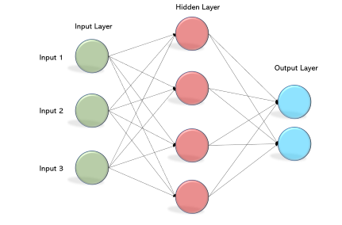
\includegraphics[height=6.5cm]{figures/MLP Network Diagram Aidan.png}
  \caption{Architecture of an MLP model.}
  \label{fig:MLP_Architecture}
\end{figure}
 
The team settled on researching two different neural network types and determining how they function, and how they could be used to predict the aerodynamic forces. I decided to focus on a Multilayer Perceptron (MLP) model, which is made up of input, output and hidden layers, where the hidden layers allow the network to handle nonlinear problems. The different layers are connected by a series of neurons that each take an input and  processes it to produce an output. Each neuron has a weight that determines importance, and these weights are summed and passed through an activation function, which introduces nonlinearity to the function.
 
\subsection{Training Data}
To build the network, I made a test network that can predict the coefficient of lift, coefficient of drag, pressure drag coefficient, and the pitching moment coefficient from the angle of attack, Reynolds number, and the top and bottom transition points of various airfoils. I used a database of NACA airfoils that I gathered from "splinecloud.com" which provided a large database of various NACA airfoils and the necessary input and output parameters for the network, and compiled them into a single excel file that contained over 66,000 individual samples of data across 619 different airfoils. This excel sheet listed out all the parameters required for the network, and was also used by Wade Schnurr for his work on the Long Short-Term Memory (LSTM) model that was occurring simultaneously with my model.
 
\begin{figure}[htbp]
  \centering
  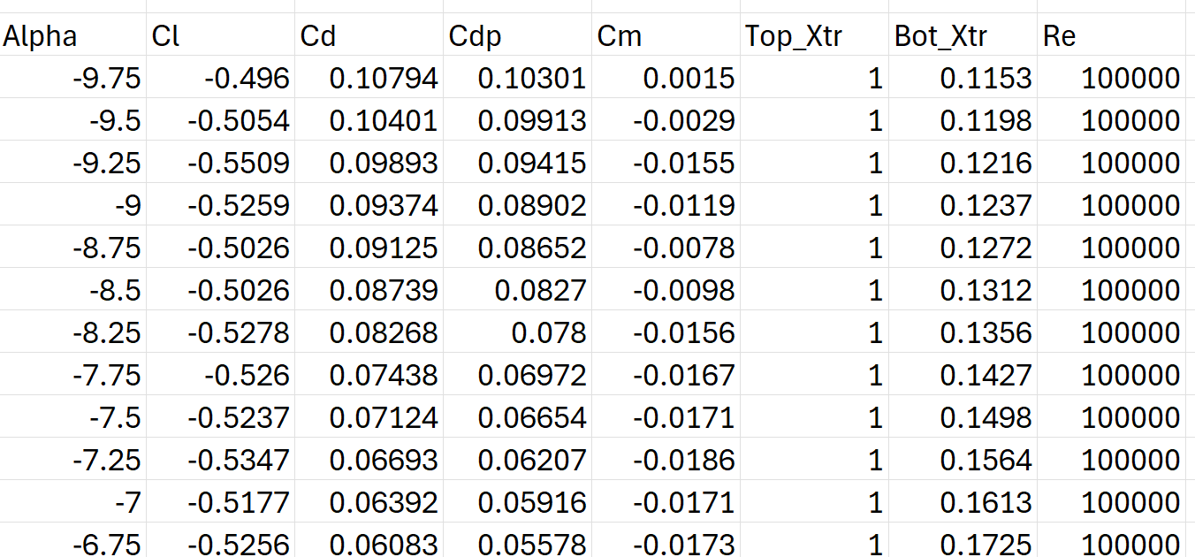
\includegraphics[height=6.5cm]{figures/Training Data Aidan.png}
  \caption{Samples of NACA Airfoil Training Data.}
  \label{fig:NACA_Airfoil_Training_Data}
\end{figure}
 
\subsection{Model and Results}
 
\begin{figure}[htbp]
  \centering
  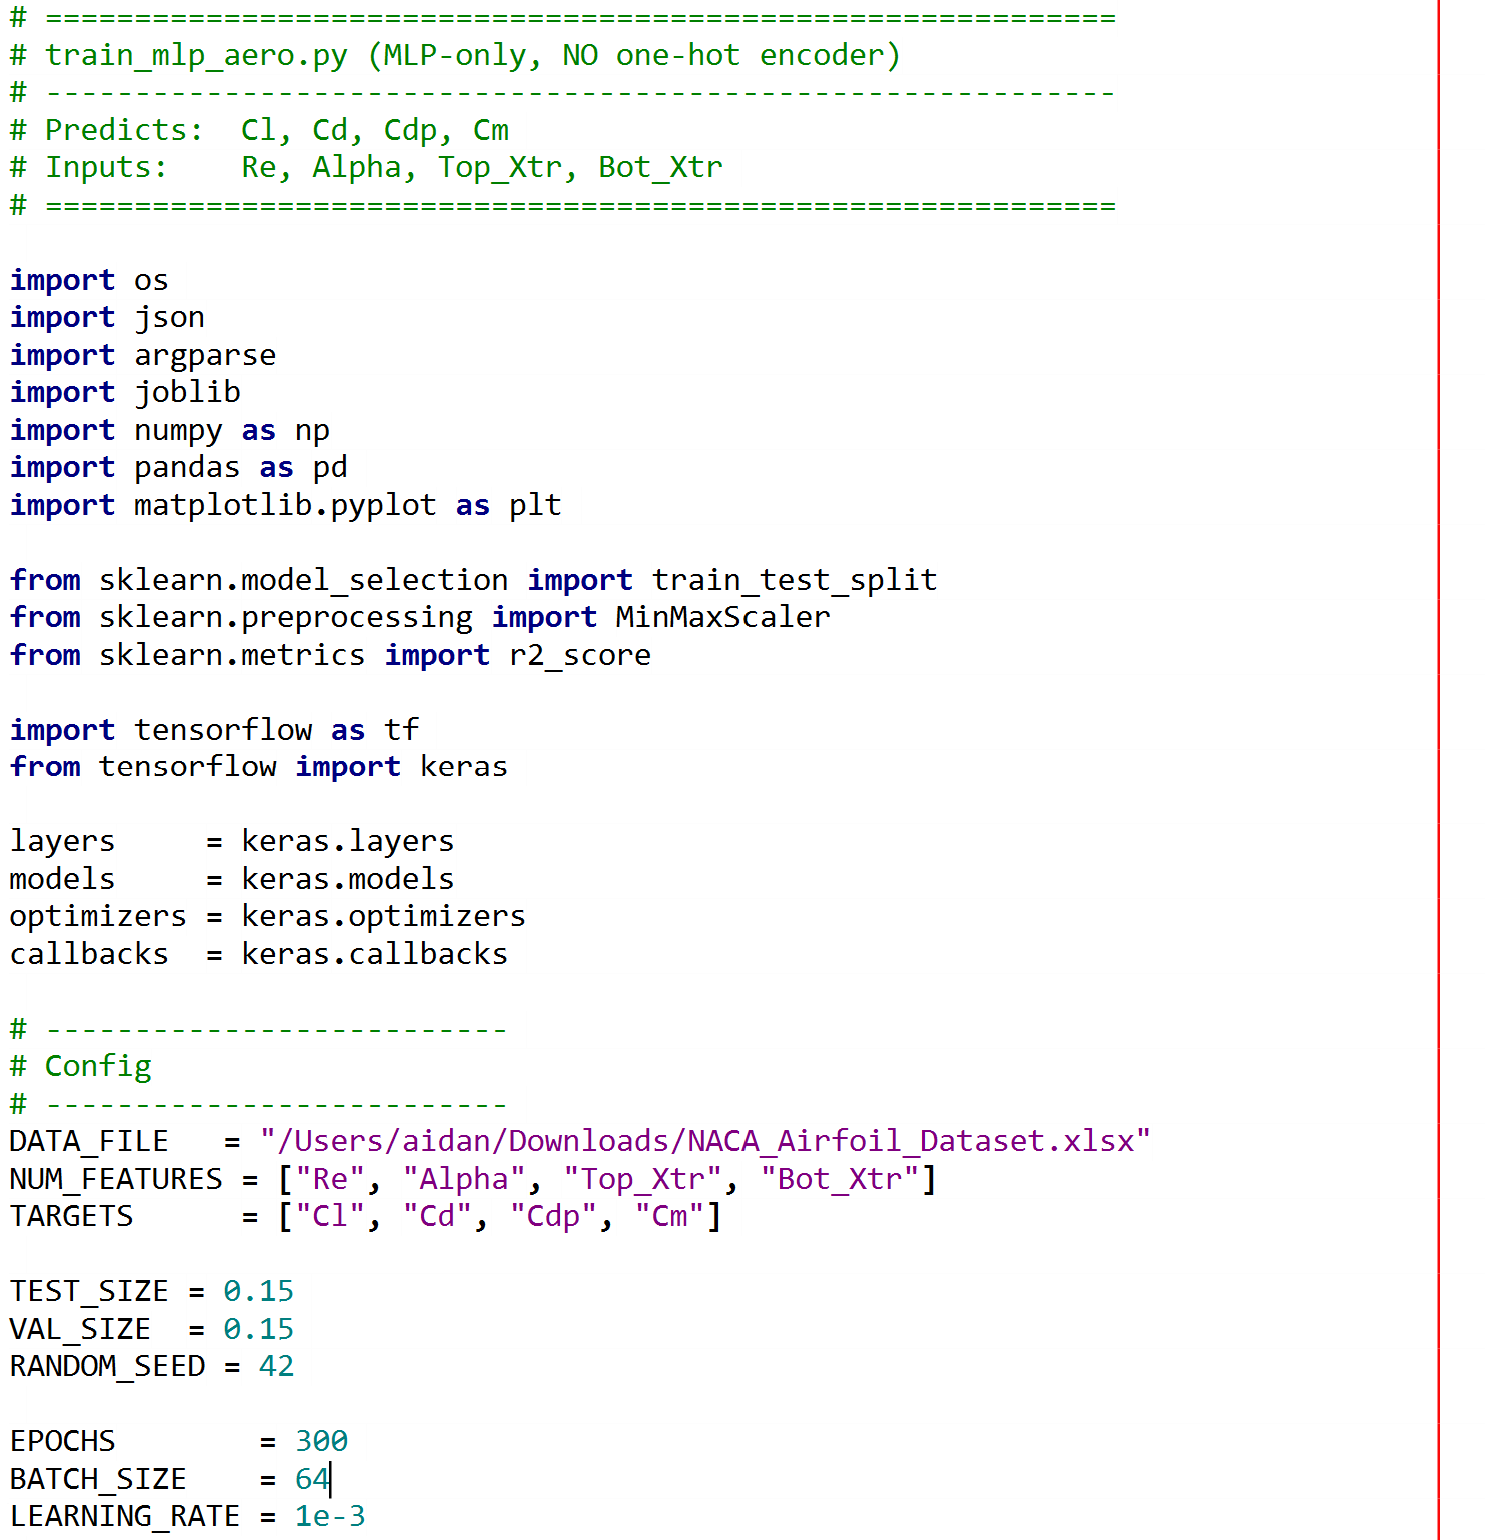
\includegraphics[height=10cm]{figures/Aidan Code Image 1.png}
  \caption{Sample of the MLP Network Code Used in Training Model.}
  \label{fig:MLP Code}
\end{figure}
 
The network that I used had three hidden layers due to the complexity of the network with 4 inputs and outputs, and included 452 neurons, which are 256, 128 and 64 in the hidden layers, and 4 for the input layer as is standard for MLP networks. The network included a Rectified Linear Unit (ReLU) activation function, which outputs 0 for negative inputs and the input itself for positive inputs, which is useful for modeling complex relationships in data. The network also has a dropout function, which randomly deactivates neurons during training in order to prevent over-fitting.
 
\begin{figure}[htb]
  \centering
  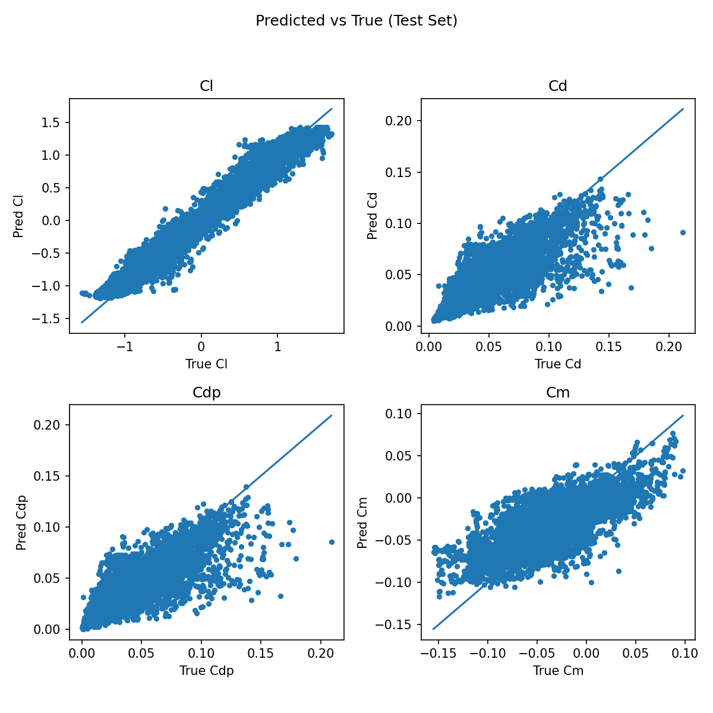
\includegraphics[height=6.5cm]{figures/Predicted vs True Aidan.png}
  \caption{Predicted vs. Real Values of Parameters.}
  \label{fig:Predicted_vs_Real}
\end{figure}
 
\begin{figure}[htbp]
  \centering
  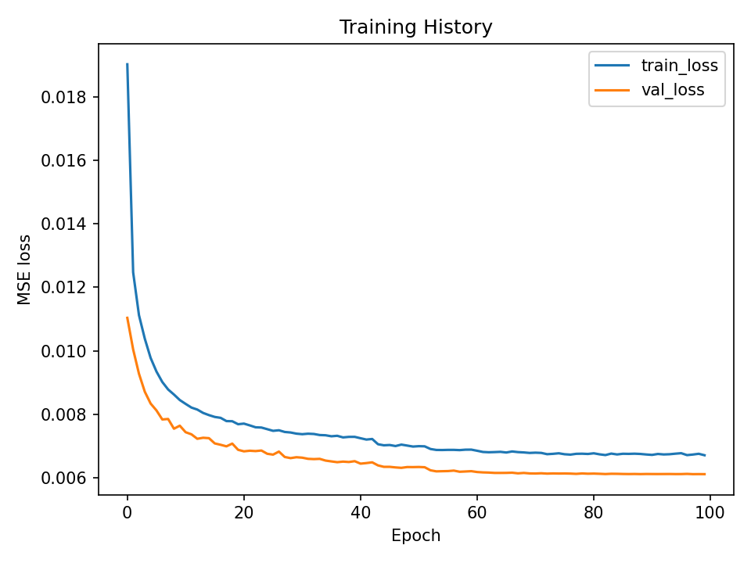
\includegraphics[height=6.0cm]{figures/Training and Validation Loss Aidan.png}
  \caption{Training and Validation Losses throughout Training}
  \label{fig:Training_and_Validation}
\end{figure}
 
\begin{table}[htbp]
    \centering
    \begin{tabular}{|c|c|}
        \hline
        Accuracy Type & Accuracy Percentage \\ \hline
        Training Accuracy & 90.4805 \\ \hline
        Validation Accuracy & 91.8836 \\ \hline
        Test Accuracy & 96.304 \\ \hline
    \end{tabular}
    \caption{Training, Validation, and Test Accuracies}
    \label{tab:four_by_two}
\end{table}
 
\newpage
The training, validation and test accuracies were found to be 0.904805, 0.918836 and 0.963504 respectively. The accuracies can be increased with more epochs and a smaller batch size, where 100 epochs were used with a batch size of 64. Overall, this is good progress for the network.
 
\subsection{Plan for Winter Semester}
Next semester, the team will focus on using the model to predict the three-dimensional aerodynamic forces acting upon the flapping wings. Once the model is accurate enough, the input parameters will have to be determined and sufficient data will have to be collected by the rest of the ATPW team in order to be able to predict these forces.